\chapter{I Asked Robert Herjavec How He Made \$500 Million}

This chapter follows Lecture 33 of the School of Hard Knocks interview series, curated by LazyingArt LLC. The lecture opens by throwing large numbers at us before it gives us the mechanism that makes those numbers intelligible. We hear of company sales, annual earnings, luxury markers, and finally the sentence that organizes the whole chapter: one can be rich without yet being wealthy. The Beverly Hills street interviews that follow are therefore not disposable scenery. They are a mechanism bank. By the time Robert Herjavec arrives, the lecture has already assembled fragments about action, regret, screening, differentiation, competition, and sales, and Herjavec's own interview converts those fragments into a clearer arithmetic of ownership, exits, and durable assets.

\section{The Teaser Problem}

The opening montage does not begin with explanation. It begins with outcomes: one company sold for \$30 million, another sold for many hundreds of millions, a television network sold to News Corp, a year with roughly \$17 million in earnings, and the compact distinction, ``I'm not rich. I'm wealthy.'' We should keep the order of presentation because the lecture wants the puzzle first and the doctrine later.

To keep the arithmetic clean, we introduce a small amount of notation.

\begin{definition}
We write
\begin{align}
Y &= \text{annual income},\\
A &= \text{an owned asset or business},\\
V(A) &= \text{the realizable sale value of }A,\\
W &= \text{wealth as durable command over assets and retained gains}.
\end{align}
\end{definition}

The teaser is then compressed by the claim
\begin{equation}
W \not\equiv Y.
\end{equation}
A high yearly income is one kind of success, but the lecture is already pointing toward another kind, namely value that sits in an owned thing and can later be sold:
\begin{equation}
W \sim V(A) + \text{retained gains}.
\end{equation}
This is not yet the whole story, and the lecture does not want us to solve it too soon. It wants first to move through a field of examples.

\section{Beverly Hills as a Wealth Field}

The host arrives in Beverly Hills with a declared purpose: before meeting Herjavec, he will ask the people already moving through this wealthy environment what they did to become wealthy. We should read this as method, not as atmosphere. The neighborhood becomes a sampling device. Instead of beginning with a single authority, the lecture begins with multiple local operators, each of whom contributes one fragment of a larger commercial grammar.

Three distinct grammars appear in the prelude:
\begin{itemize}
\item wealth by exit, where a company, network, or product line is eventually sold;
\item wealth by operation, where a founder organizes people, process, and market timing;
\item wealth by positioning, where the operator sees demand, differentiates an offer, and turns competition into a signal rather than a deterrent.
\end{itemize}

That is why the prelude must remain in the chapter. It lowers the altitude. Before the lecture gives us a clean sentence about capital gains and saleable value, it lets us hear how such value sounds in the mouths of operators whose businesses are fitness, education, direct response, media, promotion, and investing.

\section{Action, Health, and the Cost of Not Acting}

The first street case is Body by Jake, and the lecture does something important here: it moves from visible wealth to invisible cost. Jake is introduced not by a theory but by a life pattern. He has been an entrepreneur since youth; he looks physically disciplined; he says that health is wealth; he emphasizes risk-taking; and he places unusual weight on the spouse or partner who stands with the entrepreneur through uncertainty.

The conversation then turns away from glamour and toward regret. Jake's point is not that entrepreneurship guarantees victory. In fact, he states the contrary: one wins some and loses some. What matters is not the fantasy of an unbroken streak but the refusal to live with unrealized attempts. He gives the lecture its first strong moral-commercial line: graveyards are full of valuable ideas that never became companies because their owners never acted on them.

\subsection{Question \& Answer}

\paragraph{Question.} What is the cost of not acting on an idea?

\paragraph{Answer.} In this lecture the cost is not measured only in foregone cash. The deeper cost is deferred self-judgment. The entrepreneur who reaches sixty or seventy still carrying the memory of ideas never attempted has not merely missed upside; he has accumulated regret. The lecture therefore treats action as protective. To take the shot is already to escape one category of failure.

Jake's later remarks reinforce the same point from another side. He recalls selling a television network to News Corp, but when pressed for a terminal principle after losing his house in the Palisades fire, he does not answer with property, cars, or sale multiples. He answers with a question: what are you made of? Here the lecture sharpens a distinction it will return to later. Material outcomes are real, but they are not the deepest diagnostic. The operator must still survive the stripping away of appearances.

His commercial motto, ``No is halfway to yes,'' belongs here as well. It is not a theorem. It is an action rule. The entrepreneur hears refusal not as terminal information but as intermediate resistance.

\section{Screening, Crisis, and Product Differentiation}

The next operator introduces himself as an investor in education. The transcript renders his institution as Theoria Technical College in Carlsbad, California. Whether or not we verify the exact spelling elsewhere, the logic of the interview is clear: he owns and buys educational institutions, and he describes his investment screen in a three-part form.

\begin{equation}
I_{\mathrm{people}} + I_{\mathrm{processes}} + I_{\mathrm{profitability}} \lesssim 2,
\qquad
I_{\bullet} \in \{0,1\}.
\end{equation}

This is only a schematic rendering of his spoken claim that most companies have two of the three. But it is a useful one. The underwriting problem is no longer ``Is this company perfect?'' The problem becomes: which leg is missing, and can the investor add value to that missing leg?

\begin{figure}
\centering
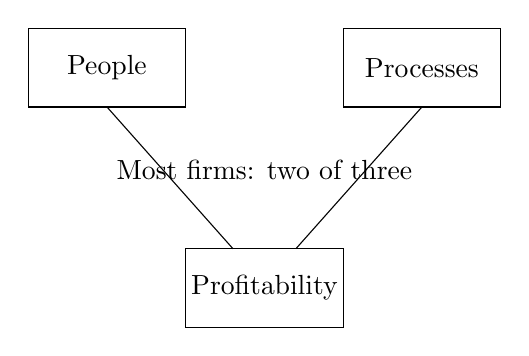
\begin{tikzpicture}
\draw (-3,1) rectangle (-1,2);
\node at (-2,1.5) {People};
\draw (1,1) rectangle (3,2);
\node at (2,1.5) {Processes};
\draw (-1,-1.8) rectangle (1,-0.8);
\node at (0,-1.3) {Profitability};
\draw (-2,1) -- (-0.4,-0.8);
\draw (2,1) -- (0.4,-0.8);
\node at (0,0.2) {Most firms: two of three};
\end{tikzpicture}
\end{figure}

The lecture immediately attaches a timing rule to this screen. When the pandemic hit and the world ``crashed,'' the operator says he doubled down. In words, fear and opportunity are positively correlated for the investor who is willing to act. This is not a law of nature, but it is a recurring entrepreneurial conviction in the lecture: the crowd's retreat may reveal a wider field for the operator who can still move.

He then offers a management heuristic through the ``Obama effect'': surround oneself with smart people, speak last, let others contribute, and build a room in which the leader is not required to be the smartest person present. Notice the continuity with the previous section. Action remains central, but now action is organizational rather than merely personal.

After a sponsor interruption, the lecture returns to a final warm-up case in direct response and promotion. This operator is associated with health products, the first ``Herbal Viagra,'' Fit TV, telemedicine, and a reading discipline centered on books such as \textit{Think and Grow Rich} and Dan Kennedy's \textit{The Ultimate Sales Letter}. What matters for the chapter is not bibliography for its own sake, but the mechanism he attaches to product finding and product standing.

He says the entrepreneur must keep eyes open, read, think, talk to people, and network. He then makes a stronger market claim: competition is not itself a reason to stay out.

\begin{equation}
n_{\mathrm{competitors}} \uparrow \quad \Rightarrow \quad D_{\mathrm{market}} \uparrow
\end{equation}

Again, this is only a heuristic, and the lecture immediately limits it. Competition proves activity, but not necessarily our success inside that activity. That is why the next step is differentiation. The product has to be distinct enough to matter. In his own case, the route was not merely entering a crowded market, but finding an unusual herb-processing angle, pairing it with media, and making the offer legible to the buyer. Crowded market plus differentiated offer: that is the real pair.

\section{Rich, Wealthy, and the Arithmetic of Exit}

Now Herjavec arrives, and the lecture finally cashes the opening check. The host introduces him through cyber, technology, and business scale, but the important move is conceptual, not biographical. Asked what he saw early, Herjavec answers with the chapter's cleanest contrast:
\begin{align}
\text{follow a trend} &\to \text{get rich},\\
\text{create a trend} &\to \text{get wealthy}.
\end{align}

We should read this in the strict order given. To follow a trend is to monetize participation. To create a trend is to monetize control, early ownership, or category-making advantage. The sentence is not yet about arithmetic, but it is already about who gets paid as a participant and who gets paid as an owner.

He then reframes motivation. Mark Cuban, he says, wanted to be rich at twelve. Herjavec wanted not to be poor. The lecture matters here because it moves from aspiration to escape velocity. One can be moved not only by the desire for excess, but also by refusal of prior conditions. That leads directly to the lecture's action axiom:
\begin{equation}
S_{t+1} \approx S_t
\qquad
\text{when}
\qquad
\Delta a_t = 0.
\end{equation}
This is only an editorial shorthand for the spoken line, ``Nothing changes if nothing changes,'' but it captures the logic exactly enough for our purposes. If the action variable does not move, the state variable remains substantially the same.

\subsection{Question \& Answer}

\paragraph{Question.} Why can a person earn a very high income and still fail to become truly wealthy?

\paragraph{Answer.} Because annual income and ownership value are not the same thing. Income can make one very rich, but the lecture insists that wealth jumps when the operator owns something that can later be sold. The sale event is qualitatively different from a large paycheck. It is not merely more income. It is the realization of value stored in an asset.

Herjavec makes the distinction explicit in numbers:
\begin{align}
M_{\mathrm{peak}} &= Y + G_{\mathrm{exit}},\\
M_{\mathrm{peak}} &\approx \$500\text{M},\\
Y &\approx \$18\text{M}.
\end{align}
Here \(M_{\mathrm{peak}}\) is his biggest money year, \(Y\) is income on an income basis, and \(G_{\mathrm{exit}}\) is the gain associated with selling a business. The lecture itself supplies the structure even if it does not provide a line-by-line tax statement.

\paragraph{A worked decomposition.} At the level of lecture arithmetic, the derivation is straightforward.
\begin{enumerate}
\item Start from the identity \(M_{\mathrm{peak}} = Y + G_{\mathrm{exit}}\).
\item Insert the lecture values \(M_{\mathrm{peak}} \approx \$500\text{M}\) and \(Y \approx \$18\text{M}\).
\item Subtract to isolate the exit component.
\end{enumerate}
Thus
\begin{align}
G_{\mathrm{exit}}
&\approx M_{\mathrm{peak}} - Y \\
&\approx \$500\text{M} - \$18\text{M} \\
&\approx \$482\text{M}.
\end{align}
The exact split is not given in the transcript, so we keep this as a schematic example. But the point is decisive: the enormous year is not salary-sized. It is exit-sized.

\begin{figure}
\centering
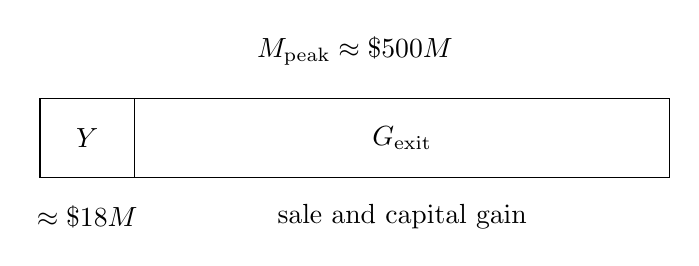
\begin{tikzpicture}
\draw (0,0) rectangle (8,1);
\draw (0,0) rectangle (1.2,1);
\node at (4,1.6) {$M_{\mathrm{peak}} \approx \$500\text{M}$};
\node at (0.6,0.5) {$Y$};
\node at (4.6,0.5) {$G_{\mathrm{exit}}$};
\node at (0.6,-0.5) {$\approx \$18\text{M}$};
\node at (4.6,-0.5) {sale and capital gain};
\end{tikzpicture}
\end{figure}

This figure is schematic rather than to scale. Its purpose is simply to preserve the lecture's distinction between a flow and a realization. Once that distinction is made, the opening teaser becomes mathematically legible. One can earn a lot. One becomes wealthy when one builds, owns, and eventually exits something of far greater value.

\section{Recovery, Sales, and Relationship Capital}

Once the arithmetic is clear, the lecture refuses to become clean. It turns immediately to betrayal. Herjavec recalls discovering that a sales manager had been stealing from him by routing orders through his own side company. The important lesson is not that successful people avoid bad days. The lecture says the opposite. What matters is recovery speed. Barbara Corcoran's contribution here is that the true variable is the duration of misery, not the absence of misery. Herjavec cries, feels sorry for himself, and then gets up and goes again. Elon Musk's language of ``eating glass and staring into the abyss'' is used to name the same terrain from a harsher angle.

The next move is financial doctrine, and it remains explicitly attributed. Charlie Munger, as reported by Herjavec, advises never selling a house. Herjavec translates this into a hold-horizon rule:
\begin{equation}
H_{\mathrm{RE}} \ge 10 \text{ years}
\quad \Rightarrow \quad
\Pi_{\mathrm{RE}} > 0.
\end{equation}
He immediately adds the true danger:
\begin{equation}
H_{\mathrm{RE}} < 10 \text{ years}
\quad \text{with forced sale from liquidity pressure}
\end{equation}
is where the trouble begins. The enemy is not simply real estate volatility. The enemy is the loss of time.

The lecture then pivots into sales, and here it becomes almost procedural. Before one teaches someone to sell, one must ask who the buyer is. The largest error in selling is to reuse one pitch on every person. That is why we can write
\begin{equation}
p_{\mathrm{close}} = p(N,P),
\qquad
\text{with } N \text{ discovered before } P.
\end{equation}
The notation is schematic, but the sequence is faithful: first identify need, then pitch.

\subsection{Question \& Answer}

\paragraph{Question.} What actually makes someone willing to buy from us?

\paragraph{Answer.} The lecture gives a two-part answer. First, we must match the offer to a real need. Second, we must affect the buyer emotionally. Herjavec says later, ``Sell joy,'' and the phrase is not ornamental. It completes the sales model. A buyer does not receive only information. A buyer also receives a feeling about the person, the interaction, and the future that the interaction seems to promise.

From sales the lecture moves naturally to relationship capital. Herjavec rejects the lazy formula that success is mainly ``who you know.'' His counterclaim is harder and more constructive. If one begins with little money and few connections, one must become the kind of person other people want to know. That gives us the chapter's relationship update rule:
\begin{equation}
C_{t+1} = f(C_t, V_t),
\end{equation}
where \(C_t\) is connection capital and \(V_t\) is visible value delivered to others. The mechanism is not begging for access. It is building enough value that access starts to move toward us.

The lecture then names obsession as the common trait of the ultra-successful. Passion is too soft and too temporary. Obsession lasts. Herjavec links this to a peculiar kind of vision: the ability to see not only the world as it is, but the world as one wants to make it. At this point the recurring health motif reappears. The highest flex of wealth, he says, is being in shape. The argument is no longer comic. If money does not support health, then its meaning is diminished.

The next distinction concerns starting conditions:
\begin{align}
K_0 > 0 &\Rightarrow \text{use capital as leverage and barrier to entry},\\
K_0 \approx 0 &\Rightarrow \text{favor e-commerce and brand-building}.
\end{align}
Commercial buildings, data centers, and land belong to the first branch. Brand-led e-commerce belongs to the second. The point is not that one branch is nobler, but that strategy should follow capitalization.

The lecture immediately adds another ranking:
\begin{equation}
(\text{good operator},\text{bad idea})
\succ
(\text{bad operator},\text{good business}).
\end{equation}
Herjavec says this in plain language: he invests in people over ideas. A strong person can improve a weak idea. A weak person can ruin a strong business.

The ``man in the t-shirt'' anecdote with Mark Cuban pushes the same point through social signaling. The man in the t-shirt is dangerous because he no longer has to dress to impress. The direction of selling has reversed. He is not selling the room. The room is selling him. This is an important late-stage status marker in the lecture: freedom from signaling is itself evidence of accumulated position.

From there the lecture turns to AI. If Herjavec lost everything but kept his contact book, he says he would start an AI company. More specifically, he favors the data infrastructure side over the merely consumer side, and he recommends training an AI model to one's own working style. The advice is practical rather than metaphysical: do not merely use the tool; tune the tool until it begins to operate in your own pattern.

The final doctrine then widens from business technique to human presence. ``Sell joy.'' ``It's not what you say, it's how you make people feel.'' A priest tells Herjavec that nothing in life is as fascinating as another human being, and Herjavec brings that line back into sales. Everybody has a story. Everybody has interiority. To approach others with open fascination is not only humane; it is commercially effective. The lecture ends, therefore, where it began to move in the prelude: wealth may be built through assets, but business remains a deeply interpersonal practice.

\section{Summary}

The chapter begins with conspicuous outcomes and ends with a cleaner mechanism. Wealth is not the same as a large income. The decisive jump comes when an operator owns something of value and can sell it. Around that core arithmetic the lecture layers a broader operating method: act before regret hardens, screen companies by people, processes, and profitability, treat crisis as a revealing moment, differentiate in crowded markets, hold real estate long enough to survive liquidity pressure, discover need before pitching, build access by providing value, and remember that the final medium of business is still human feeling. The lecture's progression is therefore exact: first the numbers, then the field evidence, then the arithmetic, and finally the discipline required to live inside that arithmetic without being consumed by it.